\section{Background}
\label{sec:background}

\subsection{Mobile Device Authentication Through Body Movements}


%\begin{comment}
%\end{comment}

%Authentication mechanisms for wearable devices can broadly be divided into two
%categories: (i) {\em Direct} authentication, where the users can directly
%authenticate themselves to their wearable device using the input/output
%interface and/or using signatures generated from the sensors available on the
%device, and (ii) {\em Indirect} authentication, where a secondary device --
%typically the user's smartphone -- is used as a medium for authentication.
%Today's commercially available wearable devices predominantly use the latter
%approach where users login to their wearable devices through their smartphone
%-- using a PIN or an email account.
%%A select few gadgets, for example the Google Glass or fitbit, require the
%%users to register their device to their user specific accounts (gmail for
%%Google Glass), which can also be perceived as an indirect mechanism for
%%authentication.
%Unlike the indirect approaches, that require users to have multiple devices, direct
%mechanisms only rely on the wearable device by leveraging the inbuilt interfaces and sensors on the
%wearable device.

%%One form of direct authentication is the well-known
%%the PIN code approach, however, its effectiveness is only limited to the PIN
%%being safe-guarded by the user. A slightly more effective approach would be
%%to use a randomly generated code for the user, similar to the RSA
%%%keys~\cite{},but that would require a secure and stable wireless connection
%%%to the server.
%The fact that wearable devices relate significantly to ``what we wear" on the
%human body, biometrics can play a key role for direct authentication to
%wearable
%devices.

%Biometrics allow a system to identify a user based upon ``who you
%are" (i.e., her physiology) instead of ``what you
%have'' (i.e., ID cards) or ``what you know'' (i.e.,
%passwords)~\cite{jain2004introduction,o2003comparing,yampolskiy2007motor}.
%Physiological biometrics such as DNA, ear shape, face, fingerprint,
%hand or finger geometry,
%iris, odor, palm-print, retinal scan, and voice, have been very effective and
%widely used in many prototype and commercial authentication systems.
%In addition, body shape such as body height, width, and body-part proportions
%can also be used as biometric cues to identify different
%people~\cite{collins2002silhouette}. Even characteristics such as
%body weight and fat percentage have been considered as secondary biometrics
%for authentication purposes~\cite{ailisto2006soft}.

%However, biometrics are
%not prominently used in wearable devices that are commercially available
%today, though
%there have been specific point commercial designs (e.g., Nymi~\cite{nymi}). This can be attributed to the
%fact that biometrics would require the specific hardware and sensors available on
%the wearable device. Also the overheads for physiological biometrics in
%wearable devices can be high, in both, cost for hardware as well as
%integration and computing.

%%Most of the afore-mentioned biometrics, however, require extra hardware
%%(e.g., camera) and/or processing that is too demanding for wearable devices.

A number of body-movement based authentication approaches have been proposed for mobile devices. These systems
leverage unique signatures from human behavior that may be subconscious
or in response to external stimulus or both.  For example, it has been shown that gait (e.g.~stride length, the amount of arm swing) when the user is walking or
running is a reliable identification cue, and irrespective of the
environment~\cite{stevenage1999visual}. Okumura et.al.~\cite{okumura2006study}
have shown that human arm swing patterns can be used to create signatures
to authenticate to their cell-phones. Monrose
et.al.~\cite{monrose2000keystroke} show that keystroke rhythms, when
users type on the keyboard, that include typing dynamics such as how
long is a keystroke, how far is between consecutive strokes, and how is the
pressure exerted on each key, can be used to authenticate
users. Similarly, mouse usage dynamics~\cite{jorgensen2011mouse} and touchpad
touching dynamics~\cite{bo2013silentsense,de2012touch} have also been shown to
serve as potential authentication cues.

We take the viewpoint that, in comparison to other means of authentication, body-movement based
authentication may offer great convenience. With increasing access to built-in sensors on wearables, it
has become possible to generate and infer unique behavioral signatures
specific to users. With this rationale, we design an authentication system, dubbed {\em Headbanger}, for head-worn
devices by monitoring user's unique head-movement patterns in response to an
external audio stimulus.

%\vspace{4pt}{\bf Head-movements as a behavioral biometric.}
\subsection{Using Head-movement for Authentication}
\label{subsec:headmovements}

%As such, authenticating a user involves comparing her sensor
%readings with the pre-recorded glass owner's sensor readings.
%Our design assumes that there is only one owner per glass, and we can easily
%extend our scheme to handle the cases with multiple owners.
%Figure~\ref{fig:sysarch} presents the system architecture of the \systemname,
%and in the following section, we will discuss each component of this design
%in more detail.

According to Jain et al.~\cite{jain2004introduction}, a type of body movement is useful for
authentication when it is \emph{universal}, \emph{distinctive},
\emph{repeatable}, and \emph{collectible}. %With the advancements in head-worn
%wearable computer designs, collecting head-movement
%patterns using built-in accelerometers and motion sensors has become increasingly
%accessible.
Sensors for collecting head-movement patterns are
available on most of today's head-worn wearable devices, and thus
making head movements both {\em universal} and \emph{collectible}.

In this paper, we show that free-style head movements are  \emph{distinctive} and \emph{repeatable}, especially when combined with external stimuli such as music beats. In~\systemname, music plays a crucial role in stimulating body movements such that the resulting movement pattern is natural to the user (more distinctive) and easier to remember (more repeatable). Zentner and Eerola~\cite{zentner2010rhythmic} have shown that most people move
their body as a natural response to external rhythmic stimuli such as music;
even at a very early age, infants respond to music and their movements speed
up with the increasing rhythm speed. Most adults naturally perform head
movements or hand movements when listening to a fast beat audio track~\cite{action-sound:thesis}.  When
combined with external rhythmic stimuli, we believe body movements become more
distinctive -- not only a person's movement pattern is unique, but their
response to rhythmic stimuli is also unique. In this way, the resulting
authentication system will be more dependable.

%\begin{figure*}[t]
%\begin{center}
%\begin{tabular}{ccc}
%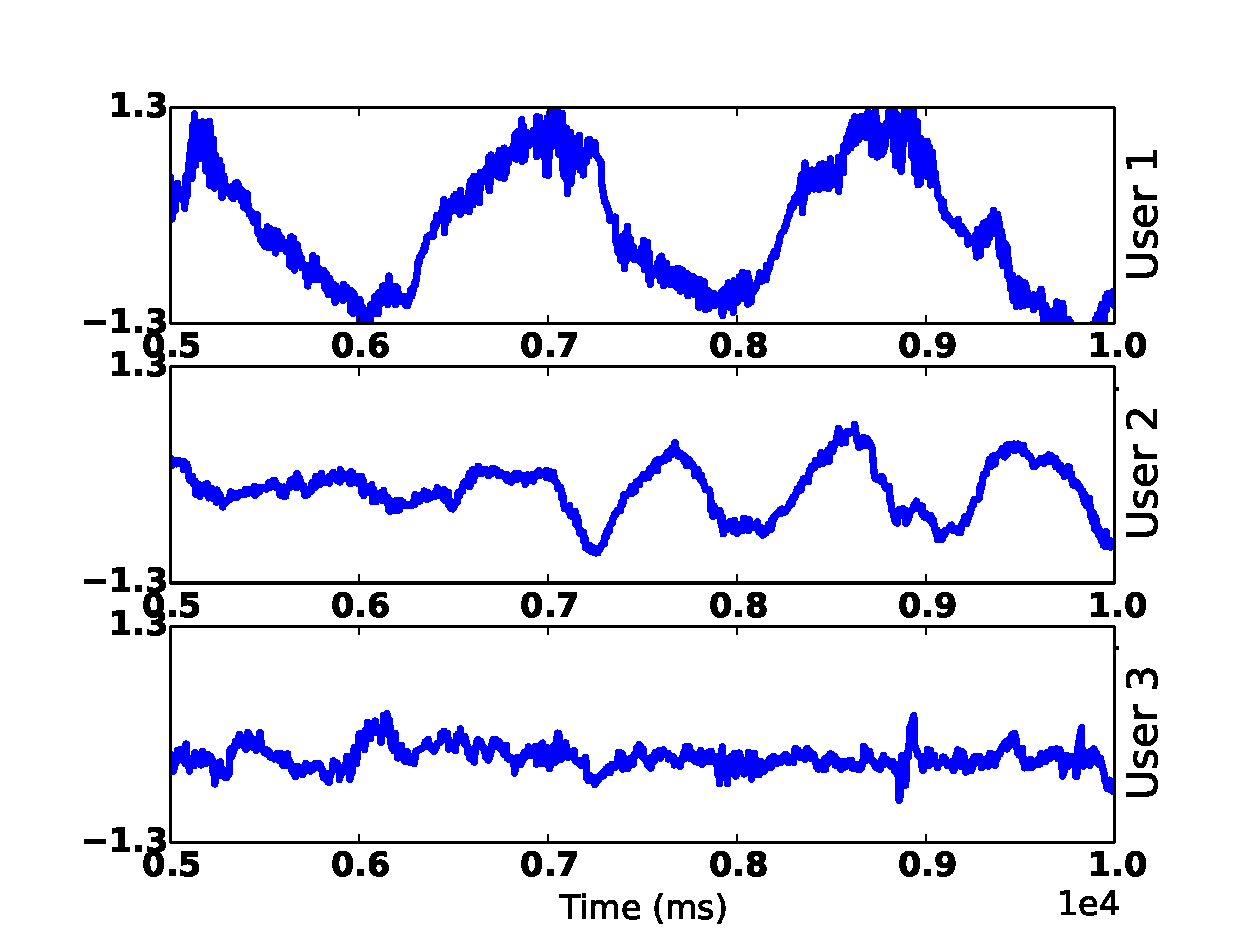
\includegraphics [width=.31\linewidth]{figure/raw_x.eps}&
%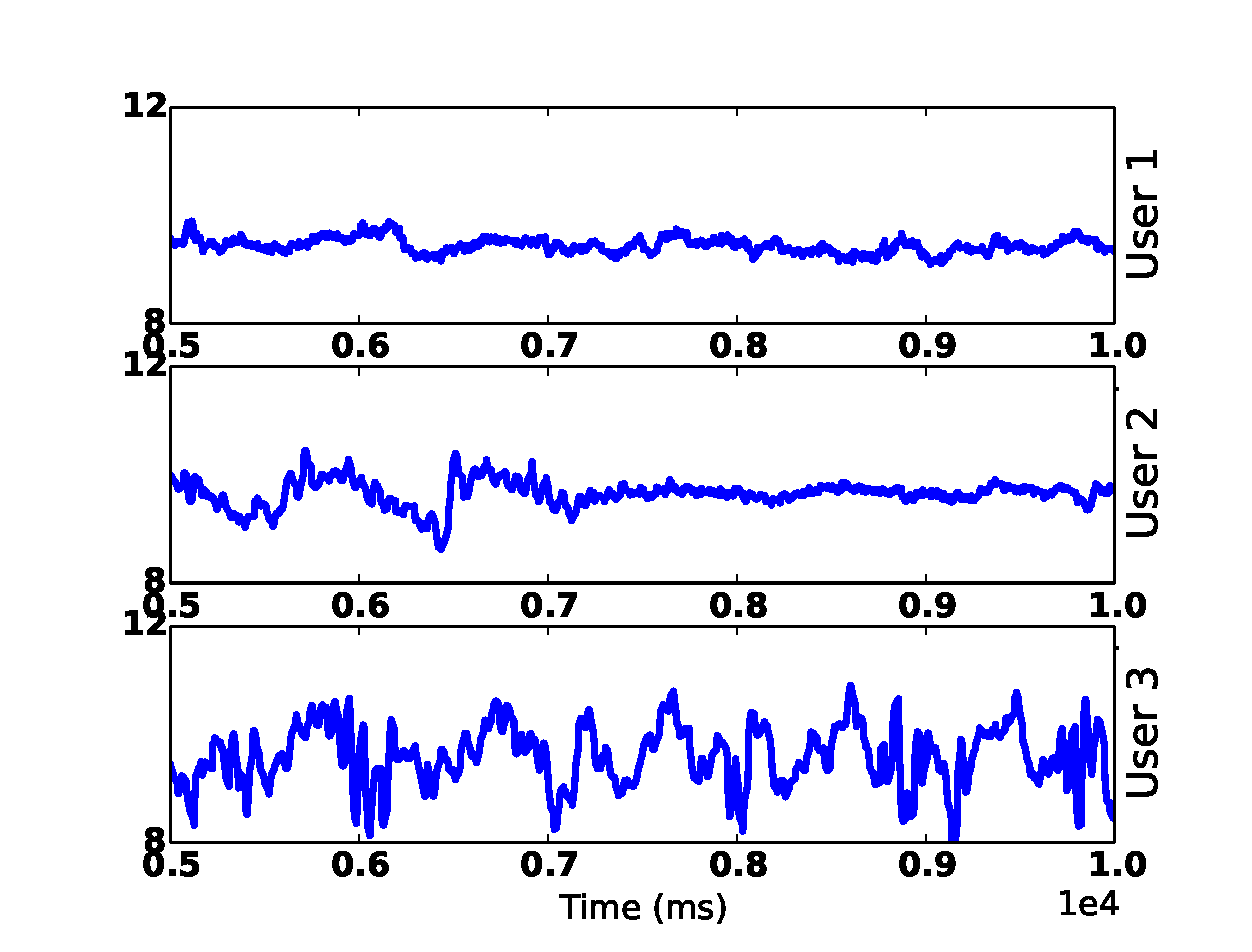
\includegraphics [width=.31\linewidth]{figure/raw_y.eps}&
%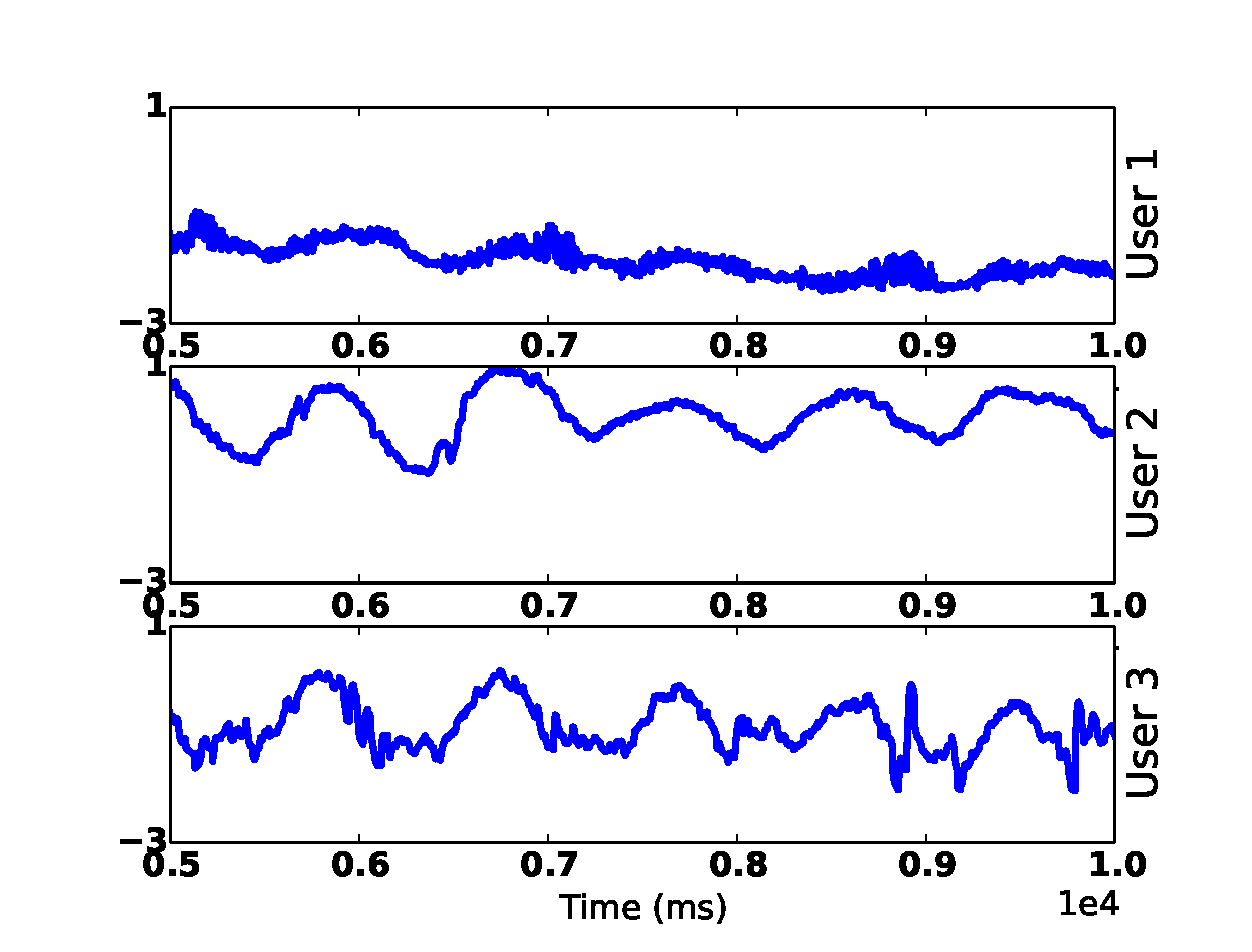
\includegraphics [width=.31\linewidth]{figure/raw_z.eps}\\
%(a) X-Axis & (b) Y-Axis & (c) Z-Axis \\
%\end{tabular}
%%\begin{tabular}{cc}
%%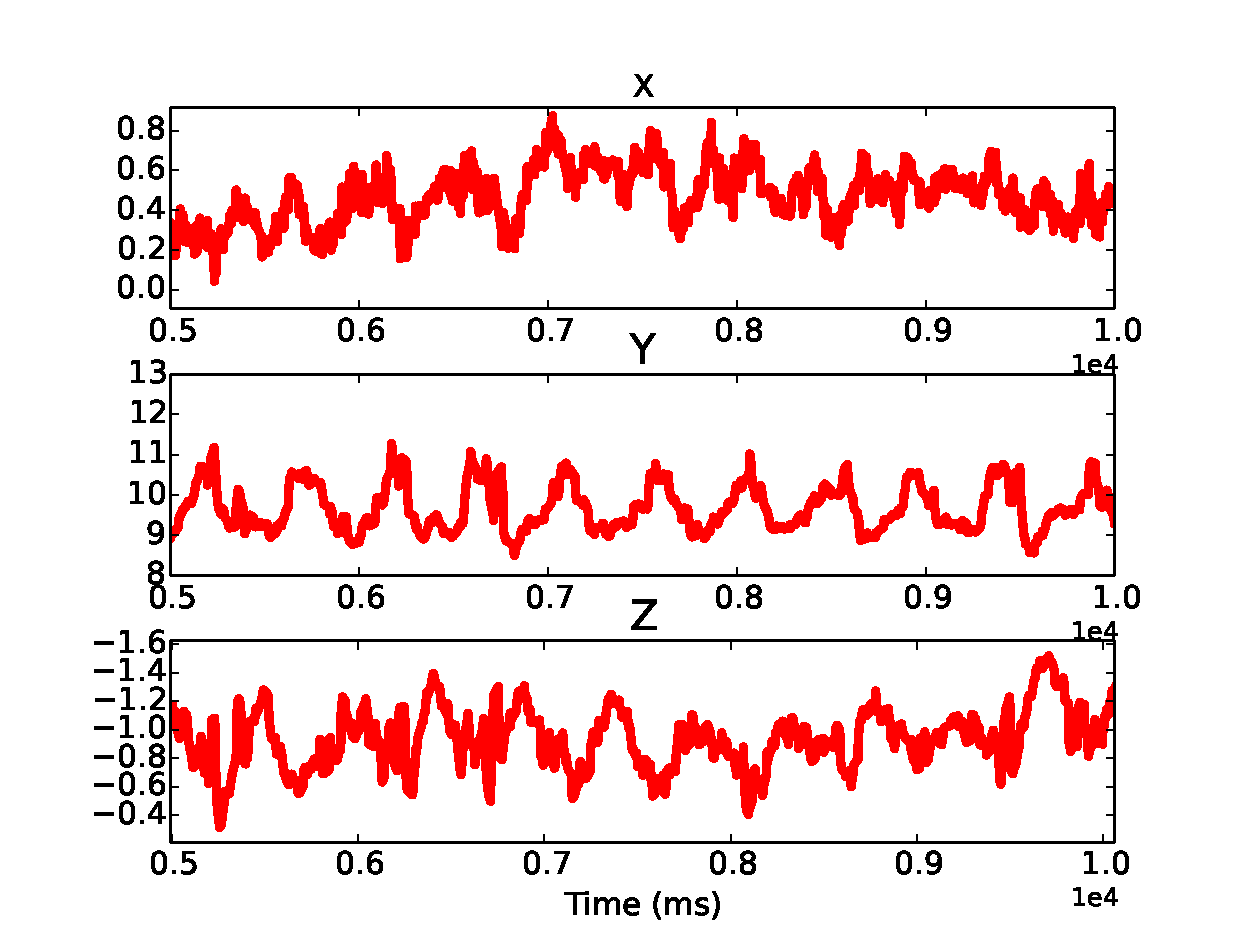
\includegraphics [width=.33\linewidth]{../fig/raw_sub4.eps}&
%%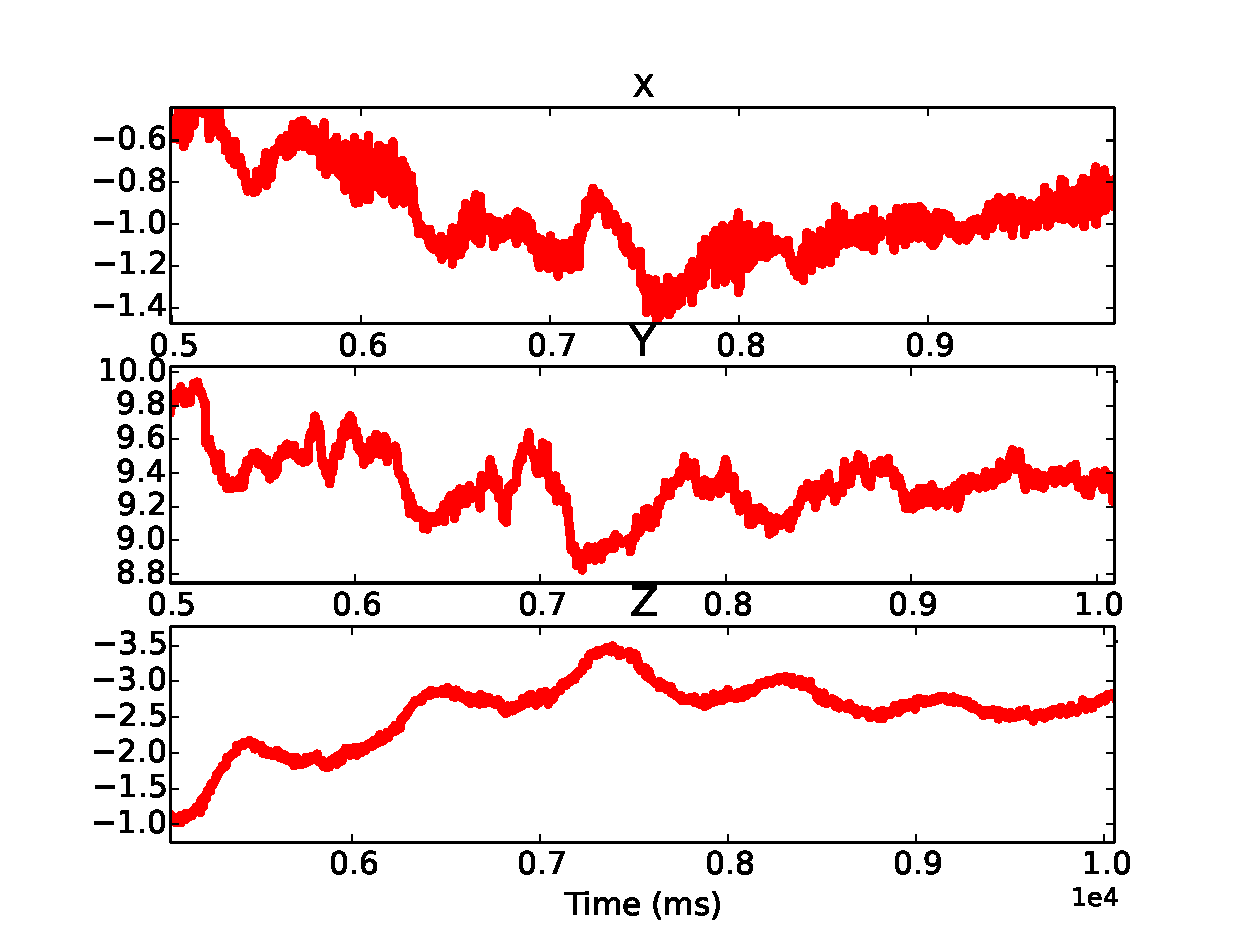
\includegraphics [width=.33\linewidth]{../fig/raw_sub5.eps}\\
%%(d) User 4& (e) User 5 \\
%%\end{tabular}
%\end{center}
%\caption{\label{fig:raw} These plots show the raw accelerometer data in the
%time domain for five different users when they move their head in response to
%the same music track wearing the same Google glass. The plots
%indicate that different users' head movement patterns appear distinctive from
%each other. The three users wore a Google Glass (in turns) and listened to a
%10 second audio snapshot of a pop song.}
%\vspace{-2pt}
%\end{figure*}

\subsection{Motivation for \systemname}
\label{subsec:motivation}
%Based on a preliminary analysis of the accelerometer signals from three Google Glass
%users, we observed (see Figure~\ref{fig:raw} (a)-(c))
%that these users {\em repeatedly} showed {\em distinctive} head-movement patterns
%(that are differentiable even through simple signal processing techniques),
%when listening to the same music beats.

%Motivated by this observation we hypothesize that head movements
%can be a good behavioral biometric characteristic to authenticate
%users to their smart glass.
%We next formally present the design of our system that
%utilizes head-movement patterns as behavioral biometric signature
%to authenticate smart glass users.



